\chapter{Math tools}
\section{Lec 2 - A recap of SR}
We will develop some of the necessary math on this framework. \\
Let's look at the Galilean Relativity. \\
Newtonian dynamics is based on three principles
\begin{enumerate}
	\item inertia
	\item $\vec{F} = m \vec{a}$
	\item action-reaction
\end{enumerate}
The first says something like \emph{An object at rest remains at rest, and an object in motion remains in motion at constant speed and in a straight line unless acted on by an unbalanced force}. \par
The second one says:
\[
	(2): \vec{F} = 0 \implies \vec{a} = 0 \implies (1)
\]

So, it seems the first principle is contained by the second, but we know that $\vec{F} = m \vec{a} $ is valid only in Inertial Frames (IF). \par
\paragraph{Galilean Relativity:} all the laws of \emph{mechanics} take the same form in every IF. (You can not distinguish two IF just by doing experiments.) \par

\begin{minipage}[t]{0.45\textwidth}
	\vspace*{0pt}
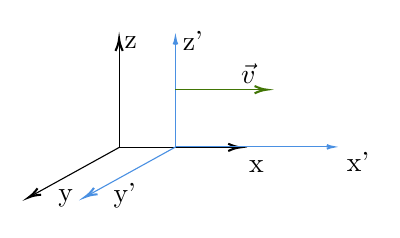
\begin{tikzpicture}[x=0.20pt,y=0.20pt,yscale=-1,xscale=1]
%uncomment if require: \path (0,514); %set diagram left start at 0, and has height of 514

%Straight Lines [id:da2496231248179689] 
\draw    (171.31,345.24) -- (171.31,151.13) ;
\draw [shift={(171.31,149.13)}, rotate = 90] [color={rgb, 255:red, 0; green, 0; blue, 0 }  ][line width=0.75]    (21.86,-6.58) .. controls (13.9,-2.79) and (6.61,-0.6) .. (0,0) .. controls (6.61,0.6) and (13.9,2.79) .. (21.86,6.58)   ;
%Straight Lines [id:da48991715239983225] 
\draw    (171.31,345.24) -- (388.33,345.24) ;
\draw [shift={(390.33,345.24)}, rotate = 180] [color={rgb, 255:red, 0; green, 0; blue, 0 }  ][line width=0.75]    (21.86,-6.58) .. controls (13.9,-2.79) and (6.61,-0.6) .. (0,0) .. controls (6.61,0.6) and (13.9,2.79) .. (21.86,6.58)   ;
%Straight Lines [id:da1967175868567953] 
\draw    (171.74,345.24) -- (9.75,434.66) ;
\draw [shift={(8,435.63)}, rotate = 331.1] [color={rgb, 255:red, 0; green, 0; blue, 0 }  ][line width=0.75]    (21.86,-6.58) .. controls (13.9,-2.79) and (6.61,-0.6) .. (0,0) .. controls (6.61,0.6) and (13.9,2.79) .. (21.86,6.58)   ;
%Straight Lines [id:da8826495136208449] 
\draw [color={rgb, 255:red, 74; green, 144; blue, 226 }  ,draw opacity=1 ]   (273.11,344.43) -- (273.11,150.32) ;
\draw [shift={(273.11,148.32)}, rotate = 90] [color={rgb, 255:red, 74; green, 144; blue, 226 }  ,draw opacity=1 ][line width=0.75]    (10.93,-3.29) .. controls (6.95,-1.4) and (3.31,-0.3) .. (0,0) .. controls (3.31,0.3) and (6.95,1.4) .. (10.93,3.29)   ;
%Straight Lines [id:da630322572196989] 
\draw [color={rgb, 255:red, 74; green, 144; blue, 226 }  ,draw opacity=1 ]   (273.11,344.43) -- (515.79,344.43) -- (555.54,344.43) ;
\draw [shift={(557.54,344.43)}, rotate = 180] [color={rgb, 255:red, 74; green, 144; blue, 226 }  ,draw opacity=1 ][line width=0.75]    (10.93,-3.29) .. controls (6.95,-1.4) and (3.31,-0.3) .. (0,0) .. controls (3.31,0.3) and (6.95,1.4) .. (10.93,3.29)   ;
%Straight Lines [id:da454762437683625] 
\draw [color={rgb, 255:red, 74; green, 144; blue, 226 }  ,draw opacity=1 ]   (273.54,344.43) -- (111.75,433.85) ;
\draw [shift={(110,434.82)}, rotate = 331.07] [color={rgb, 255:red, 74; green, 144; blue, 226 }  ,draw opacity=1 ][line width=0.75]    (21.86,-6.58) .. controls (13.9,-2.79) and (6.61,-0.6) .. (0,0) .. controls (6.61,0.6) and (13.9,2.79) .. (21.86,6.58)   ;
%Straight Lines [id:da1426561921529228] 
\draw [color={rgb, 255:red, 65; green, 117; blue, 5 }  ,draw opacity=1 ]   (273,241) -- (436,241) ;
\draw [shift={(438,241)}, rotate = 180] [color={rgb, 255:red, 65; green, 117; blue, 5 }  ,draw opacity=1 ][line width=0.75]    (21.86,-6.58) .. controls (13.9,-2.79) and (6.61,-0.6) .. (0,0) .. controls (6.61,0.6) and (13.9,2.79) .. (21.86,6.58)   ;

% Text Node
\draw (160,140) node [anchor=north west][inner sep=0.75pt]   [align=left] {{ z}};
% Text Node
\draw (385,365) node [anchor=north west][inner sep=0.75pt]   [align=left] {{ x}};
% Text Node
\draw (40,416) node [anchor=north west][inner sep=0.75pt]   [align=left] {{ y}};
% Text Node
\draw (265,130) node [anchor=north west][inner sep=0.75pt]   [align=left] {{ z'}};
% Text Node
\draw (561.63,350) node [anchor=north west][inner sep=0.75pt]   [align=left] {{ x'}};
% Text Node
\draw (140,405) node [anchor=north west][inner sep=0.75pt]   [align=left] {{ y'}};
% Text Node
\draw (387,190) node [anchor=north west][inner sep=0.75pt]   [align=left] { $\vec{v}$};
\end{tikzpicture}
\end{minipage}
\begin{minipage}[t]{0.45\textwidth}
    \vspace*{0pt}
    \[ 
    \begin{cases}
    x' = x - vt \\
    y' = y \\
    z' = z \\
    t' = t
\end{cases}\]
      \[
      t = t' = 0 \implies O = O'\]
\end{minipage} 
\bigskip

Taking the first derivative:
\begin{equation}
\begin{cases}
v_{x}' = v_{x} - v \\
v_{y}' = v_{y} \\
v_{z}' = v_{z} \\
\end{cases} \text{and for the 2\textsuperscript{nd} derivative: } \\
\begin{cases}
a_{x}' = a_{x} \\
a_{y}' = a_{y}\\
a_{z}' = a_{z}
\end{cases} \implies \vec{a}' = \vec{a}
\end{equation}
so also $\vec{F}' = \vec{F}$. And if \emph{m} is independent on the frame, we got
\begin{equation}
\vec{F}'=m \vec{a}' = \vec{F} = m \vec{a}
\end{equation}
\bigskip

Then there are Maxwell equations, people thanks to them found that EM-waves propagates with speed \emph{c} in the void. \par
But they found also that these equations were not invariant in Galilean Boosts. \par
Things started to get better when the idea of a preferred IF was ditched and Einstein decided to use Lorentz Transformations.\par

There are two postulates: \par
\begin{itemize}
	\item \emph{Relativity principle}: same as before but with \emph{physics} instead of \emph{mechanics}. \textbf{All the laws of physics ...}
	\item \emph{Speed of light}: in every IF, light propagates with constant speed, \emph{c}.
\end{itemize}
So we see that Galilean transformation become inconsistent with this, meanwhile stays valid for $\vec{v} \ll \vec{c}$.\par
As mentioned before, updated version of G. Boosts are Lorentz transformations (or Lorentz Boosts.)
\begin{equation}
\begin{cases}
	x' = \frac{x-vt}{\sqrt{1-(\frac{v}{c})^{2}}} \\
	y' = y \\
	z' = z \\
	t' = \frac{t- vx/c^{2}}{\sqrt{1-(\frac{v}{c})^{2}}}
\end{cases}
\end{equation}

To ensure the L.T. Is consistent we can perform three different checks:
\begin{itemize}
	\item $v \ll c$
	\item v = 0
	\item dimensional check
\end{itemize}
People use a notation to make the L.T. easier to write: $\gamma(v) \equiv \frac{1}{\sqrt{1-(\frac{v}{c})^{2}}} $, so it becomes
\begin{equation}
\begin{cases}
x' = \gamma (x-vt) \\
y' = y \\
z' = z \\
t' = \gamma (t- \frac{vx}{c^{2}})
\end{cases}
\end{equation}

What happens to the transformation of velocity is: (v is fixed) 
\begin{equation}
\begin{cases}
dx' = \gamma(dx -vdt) \\
dy' = dy \\
dz' = dz \\
dt' = \gamma \left(dt - \frac{v dx}{c^{2}}\right)
\end{cases}
\end{equation}
 so 
\begin{equation}
\begin{cases}
 v_{x}' = \frac{dx'}{dt'} \\
 v_{y}' = \frac{dy'}{dt^{\prime }} = \frac{dy}{\gamma \left(dt - \frac{vdx}{c^{2}}\right)} = \frac{v_{y}}{\gamma \left(1- \frac{v v_{x}}{c^{2}}\right)} \\
v_{z}' = \frac{dz'}{dt^{\prime }} = ...
\end{cases}
\end{equation}
So we see that space-time changes also along other axes.\par

Now let's talk about space-time and its parts.

\paragraph{Space-time} space-time is a manifold. For now it is a collection of (t,x,y,z), four dimensional set of all the possible values of the coordinates.
\paragraph{Event} a point of space-time.
\paragraph{World line} path of a particle in space-time. \par
\bigskip
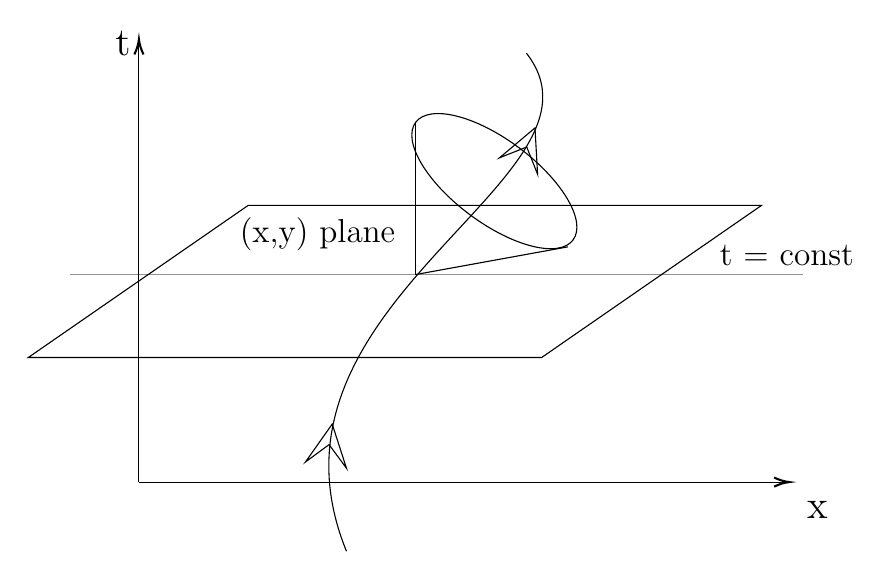
\begin{tikzpicture}[x=0.5pt,y=0.5pt,yscale=-1,xscale=1]
%uncomment if require: \path (0,393); %set diagram left start at 0, and has height of 393

%Straight Lines [id:da823225604735051] 
\draw    (120,350) -- (120,32) ;
\draw [shift={(120,30)}, rotate = 90] [color={rgb, 255:red, 0; green, 0; blue, 0 }  ][line width=0.75]    (10.93,-3.29) .. controls (6.95,-1.4) and (3.31,-0.3) .. (0,0) .. controls (3.31,0.3) and (6.95,1.4) .. (10.93,3.29)   ;
%Straight Lines [id:da9890119122071721] 
\draw    (120,350) -- (588,350) ;
\draw [shift={(590,350)}, rotate = 180] [color={rgb, 255:red, 0; green, 0; blue, 0 }  ][line width=0.75]    (10.93,-3.29) .. controls (6.95,-1.4) and (3.31,-0.3) .. (0,0) .. controls (3.31,0.3) and (6.95,1.4) .. (10.93,3.29)   ;
%Curve Lines [id:da7470868595281287] 
\draw    (270,400) .. controls (196,218.5) and (471,130.5) .. (400,40) ;
%Shape: Parallelogram [id:dp47862366089881603] 
\draw   (199,150) -- (570,150) -- (411,260) -- (40,260) -- cycle ;
%Straight Lines [id:da19245898285562835] 
\draw [color={rgb, 255:red, 0; green, 0; blue, 0 }  ,draw opacity=0.43 ]   (70,200) -- (600,200) ;
\draw   (380.57,115.65) -- (406.23,94.05) -- (408.11,127.54) -- (400.28,107.83) -- cycle ;
\draw   (240.34,335.48) -- (259.69,308.08) -- (270,340) -- (257.43,322.91) -- cycle ;
%Straight Lines [id:da33621247565465995] 
\draw    (320,90) -- (320,200) ;
%Straight Lines [id:da4519933071028329] 
\draw    (430,180) -- (320,200) ;
%Flowchart: Connector [id:dp49201896408833923] 
\draw   (320,90) .. controls (329.92,76.73) and (363.42,85) .. (394.83,108.48) .. controls (426.23,131.96) and (443.65,161.75) .. (433.73,175.02) .. controls (423.81,188.29) and (390.31,180.01) .. (358.9,156.54) .. controls (327.5,133.06) and (310.08,103.27) .. (320,90) -- cycle ;

% Text Node
\draw (191,157) node [anchor=north west][inner sep=0.75pt]   [align=left] {{\large (x,y) plane}};
% Text Node
\draw (538,177) node [anchor=north west][inner sep=0.75pt]   [align=left] {{\large t = const}};
% Text Node
\draw (101,22) node [anchor=north west][inner sep=0.75pt]   [align=left] {{\Large t}};
% Text Node
\draw (601,362) node [anchor=north west][inner sep=0.75pt]   [align=left] {{\Large x}};
\end{tikzpicture}
\bigskip

There is no notion of absolute time anymore, because now it is dependent on the frame. 
Regarding the light-cone, after the event on the ( x,y ) plane, the particle can move \emph{only} inside the light-cone, in the appropriate direction (time forward).
Now let's talk about \textbf{Clock Synchronization.} \par
It is kinda easy if in in IF. In GR it is quite subtle instead. \par

\paragraph{Example:} Be me in Origin of a RF watching my clock (A). How to define \emph{t} at another generic location (B)??

\begin{figure}
\centering
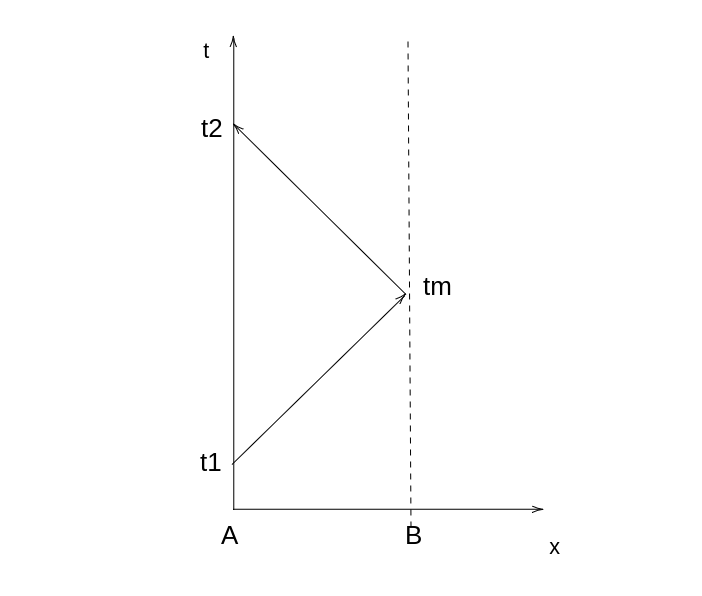
\includegraphics[width=0.5\linewidth]{imm/segnale.png}
\caption{Reception and send of the signal}
\label{imm:segnale.png}
\end{figure}

I send a light ray at time \emph{t\textsubscript{1}} to B. I get the answer on \emph{t\textsubscript{2}}. There is symmetry between the two trajectories so \[
t_{m} = \frac{ t_{1} + t_{2} }{2}. 
\]
I say to my friend on B: "set your clock to t\textsubscript{m} when you receive the signal."
So, following this methodology, each point could have its own clock.

\paragraph{Proper time:} How to define proper time? \\
\emph{t} is the time coordinate. Let's introduce the metric tensor:
\begin{equation}
	\text{the Minkowski metric tensor: } \eta_{\mu \nu } = \begin{pmatrix}
	-1 & 0 & 0 & 0 \\
	0 & 1 & 0 & 0 \\
	0 & 0 & 1 & 0 \\
	0 & 0 & 0 & 1
	\end{pmatrix} 		
\end{equation}
for a Lorentz Transformation if I have 2 events E,F.
\begin{gather*}
	\text{Frame 1: } x_{F}^{\mu } = \left( t_{F}, x_{F}, y_{F}, z_{F} \right)\\
	x_{E} = \left( ... \right) \\
	\text{Frame 2: } x_{F}^{\mu' } = \left( t_{F'}, x_{F'}, y_{F'}, z_{F'} \right) \\
	x_{E}^{\mu' } = \left( ... \right)	 
\end{gather*}
same events in 2 different frames. \\
A Lorentz Transformation connects these two events.

Be $\Delta s^{2}$ the Lorentz Invariant separation between E-F.
\begin{gather*}
\Delta s^{2} = -c \left( t_{F}-t_{E} \right)^{2} + \left( x_{F}- x_{E} \right)^{2} + \left( y_{F}-y_{E} \right)^{2} + \left( z_{F}-z_{E} \right)^{2} =\\
= -c (t_{F'}-t_{E'})^{2}  + (x_{F'}- x_{E'})^{2}  + (y_{F'}-y_{E'})^{2}  + (z_{F'}-z_{E'})^{2} \\
\Delta s^{2} = \eta_{\mu \nu } \Delta x^{\mu } \Delta x^{\nu } \\
\text{we have defined } \Delta x^{\mu } \equiv x_{F}^{\mu} - x_{F}^{\mu }, \text{with } \mu = 0,1,2,3.
\end{gather*}
From this point onward, we will use $c=1$, not a big deal, it is just a rescaling.\par

So, repeating for clarity, the Lorentz Invariant separation is
\begin{equation}
\Delta s^{2} = \eta_{\mu  \nu } \Delta x^{\mu } x^{\nu } = \eta_{\mu'\nu'} \Delta x^{\mu '} \Delta x^{\nu'}
\end{equation}
Minkowski metric tensor does not change form if we change coordinates (Cartesian coordinates, meanwhile if we use like polar ones it changes for obvious reasons.) \par

if 
\begin{align*}
	\Delta s^{2} & > 0 \text{, space-like separation} \\
		     &< 0 \text{, time-like, (it could be an actual WL for a massive particle)} \\
		     &= 0  \text{, light-like or null}
\end{align*}

Now we can define the \emph{proper time} as
\begin{gather*}
	\Delta \tau^{2} \equiv - \Delta s^{2}\\
	 \text{ or }\\
	 \Delta \tau^{2} = - \eta_{\mu  \nu }\Delta x^{\mu } \Delta x^{\nu }
\end{gather*}
to be clear, if the proper time is \emph{positive} it is time-like.

If the segment \textbf{EF} marks the begin and end of the trajectory of a massive particle, $\Delta  \tau $ is the time elapsed on a clock sitting on a RF that moves with constant speed between E and F.\par

In the moving frame $\Delta \tau = \Delta t_{*}$ where \emph{t\textsubscript{*}} is the time coordinate of the moving frame. 
In a frame where I'm at rest this is how $\Delta t^{2}$ changes:
\begin{equation}
\Delta  \tau^{2} = + \Delta t^{2} - \Delta x^{2} - \Delta y^{2}- \Delta z^{2}.
\end{equation}
